\section{Discussion}

\begin{figure}[t]
    \centering
    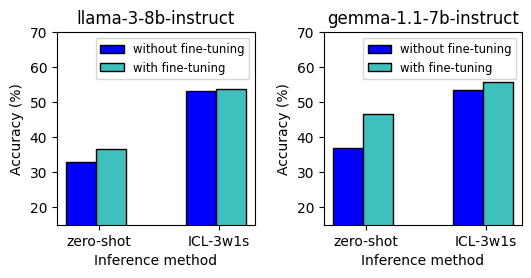
\includegraphics[width=1.0\linewidth]{figures/fig_4.png}
    \caption{Effects of in-context learning for domain adaptation scenario.}
    \label{fig:4}
\end{figure}

\subsection{In-context learning for domain adaptation scenario}
We hypothesized that if we could effectively include each domain's (i.e., private libraries) information in the LLM, the performance on RaCG would improve. The in-context learning (ICL) is one simple option when only a few annotated samples are available for unseen domains. 

In addition to \textit{zero-shot} baseline, we evaluate in-context learning with 3-way-1-shot (i.e., 1-shot for each 3 classes: answerable, partially answerable, and unanswerable), denoted as ICL-3w1s, setting. The example prompt for ICL-3w1s per domain is shown in Table~\ref{tab:2shot_prompt_netspressoeval},~\ref{tab:2shot_prompt_torchdataeval},~\ref{tab:2shot_prompt_beatnumeval},~\ref{tab:2shot_prompt_monkeyeval} of Appendix D. Each set of few-shot examples is chosen randomly. 

As we can see in Figure~\ref{fig:4}, using ICL substantially improves the accuracy compared to zero-shot inference on both with and without fine-tuning. This result implies that the RaCG benchmark prioritizes LLM learning domain information (i.e., by ICL) over learning task information (i.e., by fine-tuning).

\begin{figure}[t!]
    \centering
    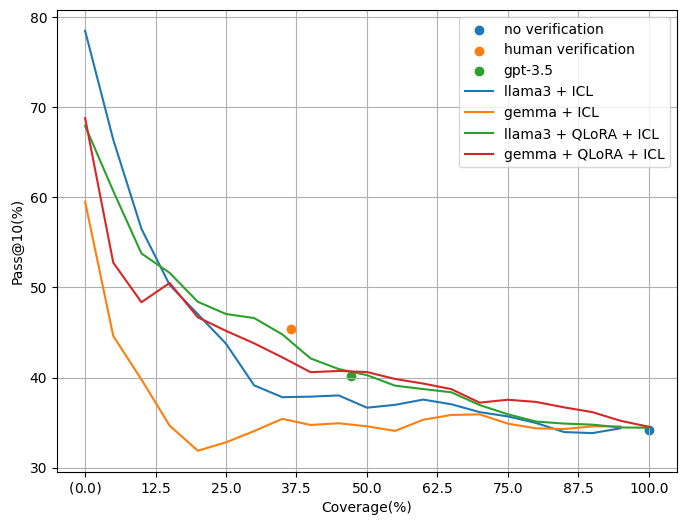
\includegraphics[width=1.0\linewidth]{figures/passAT10_only_1004.png}
    \caption{Trade-off between coverage and precision of generated code is explored across various answerability assessment models. We average the pass@k-values over 5\% bins of coverage.}
    \label{fig:coverage_VS_passATk}
\end{figure}

\subsection{Trade-off between coverage and precision of generated code}
We tested how much the average precision of code generation could be improved by introducing an answerability assessment. Only those samples classified as \textit{answerable} by the verification model were passed to the code generator, and \textit{unanswerable} or \textit{partially answerable} samples are not used by the generator.

We fix the code generator as the llama-3-8b-instruct model. The performance of the code generation was measured using the pass@k metric (k=10) \cite{chen2021humaneval}. Code generator sample \( n \geq k \) code given user query and code prefix, and then count the correct ones $c$ which pass the test code execution. If $n-k>=c$, pass@k is equal to $1-\prod\nolimits_{i=n-c+1}^{n} (1-\frac{k}{i})$, otherwise equals to 1. We used a version of the dataset with the canonical solution and test code added to the evaluation data by following \cite{zan-etal-2022-language}

Figure~\ref{fig:coverage_VS_passATk} shows the trade-off between coverage and pass@k. The coverage is defined as the percentage of the total test sample that is determined to be \textit{answerable}. This value can be controllable when we change the threshold of acceptance of the answerability assessment model. By setting a high/low threshold, we can force the code generation model to generate answers conservatively/aggressively.
Note that the coverage cannot be controllable in deterministic methods such as \textit{no verification}, \textit{human verification}, and API such as \textit{gpt-3.5-turbo API}\footnote{the API only provides token-wise top-k log-likelihood, which sometimes impossible to calculate log-likelihood of a whole sequence of 3-way responses}).

Among various verification models, fine-tuned (\textbf{QLoRA}) combined with in-context learning (\textbf{ICL}) on \textit{llama-3-8b-instruct} backbone show the best trade-off (i.e., the largest area under the curve (AUC)) compared to others.

